% AER-Article.tex for AEA last revised 22 June 2011
\documentclass[AER]{AEA}

% The mathtime package uses a Times font instead of Computer Modern.
% Uncomment the line below if you wish to use the mathtime package:
%\usepackage[cmbold]{mathtime}
% Note that miktex, by default, configures the mathtime package to use commercial fonts
% which you may not have. If you would like to use mathtime but you are seeing error
% messages about missing fonts (mtex.pfb, mtsy.pfb, or rmtmi.pfb) then please see
% the technical support document at http://www.aeaweb.org/templates/technical_support.pdf
% for instructions on fixing this problem.

% Note: you may use either harvard or natbib (but not both) to provide a wider
% variety of citation commands than latex supports natively. See below.

% Uncomment the next line to use the natbib package with bibtex 
%\usepackage{natbib}

% Uncomment the next line to use the harvard package with bibtex
\usepackage[abbr]{harvard}
\usepackage{graphicx}
\graphicspath{ {/} }
\usepackage{listings}

% This command determines the leading (vertical space between lines) in draft mode
% with 1.5 corresponding to "double" spacing.
\draftSpacing{1.5}

\begin{document}

\title{How Data Affects Decision}
\shortTitle{Short title for running head}
\author{Tanay Gahlot\thanks{Gahlot: NIT Goa, Dhavali Ponda Goa, tanaygahlot@gmail.com}}
\date{\today}
\pubMonth{March}
\pubYear{2014}
\pubVolume{I}
\pubIssue{Issue}
\JEL{}
\Keywords{}

\begin{abstract}
Whats the point in storing data?To make decisions. Due to advances in communication technology, data can transferred quickly, stored economically and analyzed efficiently. All of the above has lead to development of Reality Mining, Freakonomics, Personal Analytics, Advanced Disaster recovery solution, Social Network analysis, Human Dynamics, Social Sensing, Computational Social science and many more fields. Majority of companies have special division dedicated to analytics which try to predict cost and benefits of decision. Governance has moved to E-Governance. Battle field is becoming analytical since information is the key to win war. Mobile phones are now Smart Phones because of their computational power. City planning is done taking into considering past data. Marketing is done at a never before scale and efficiency. All decision in personal life are tested against data, even as personal a decision as Bunking a class is taken by consulting bunk affordance. Lets us jump into world of data empowered decision.
\end{abstract}


\maketitle

Honest Signal and Personal Analytics

\section{Honest Signal and Personal Analytics}
Honest signals are parameter that humans cant fake without special training therefore they make up excellent measure of human behaviour. These signals have immense potential to predict outcome of social situation like date, interview, project proposal, negotiation etc. These signals are result of extensive study done at MIT media lab by Prof. Alex Sandy Pentland, director of Human dynamics group.

What are Honest Signal?

\begin{itemize}
\item Influence: The amount of influence each person has on another in a social interaction. Influence is measured by the extent to which one person causes the other person’s pattern of speaking to match 
their own pattern. 
\item Mimicry: The reflexive copying of one person by another during a conversation, resulting in an unconscious back-and-forth trading of smiles, interjections, and head nodding during a conversation. 
\item Activity: Increased activity levels normally indicate interest and excitement, as seen in the connection between the activity level and excitement in children, or when male orangutans shake branches in order to impress potential mates. 
\item
Consistency: When there are many different thoughts or emotions going on in your mind at the same time, your speech and even your movements become jerky, unevenly accented and paced. 
The consistency of emphasis and timing is a signal of mental focus, while greater variability may signal an openness to influence from 
others. 
\end{itemize}
Humans can sense these signals unconsciously and make decision based on that. These signals were used in predicting the outcome of business plan pitching competition at MIT Sloan school of Business. By using camera and audio recorder embedded into a device known as sociometer they were able to predict the outcome of  competition with correlation r=0.6 and probability p<.01

People in real-life situations employ combinations of honest signals rather than using them individually. These combinations cluster in characteristic ways to signal the social role that the person has adopted the attitudes, intentions, and goals that characterize typical types of 
relationships between people. To illustrate how honest signals communicate social roles, I will 
start with the central interpretation of each of our honest signals. Let’s say that influence signals attention, mimicry signals empathic understanding, activity level signals interest, and consistent emphasis signals mental focus and determination (and hence inconsistent or variable emphasis signals a possible openness to influence). 
Because people have this capability for automatic signaling and response, the signaling of each person can propagate through the chains of people that make up their social network, eventually 
changing the behavior of the entire group. So when a group of people gets together, we need to consider not just the individual behaviors but also the social circuits formed by the patterns of 
signaling between them. These social circuits specify networks of dominance, obligation, friendliness, attention, and receptivity, which in turn coordinate the day-to-day behavior of the
group. 
Honest signals have evolved to coordinate individual behaviors in the midst of competition. In groups, though, competition is not just a one-on-one situation. There are instead competing coalitions supporting different alternatives, with the membership of the coalition shifting with each different question or new idea. Consequently, participants take on many different roles in quick succession, each with its own characteristic signaling display
How did primitive humans make group decisions? With only limited language skills, the decision process couldn't’t really involve logical argument. For that matter, how do ape groups decide what 
to do? With language removed from the equation, some way must still exist to gather and assess the possibilities for group action, and make group decisions that maximize rewards and minimize risk. 
There also has to be a way for each individual to know what the group decided, so that everyone can play their respective roles. This evolutionary advantage would result in the selection of the 
types of network intelligence that produced the most accurate and reliable decision making. As such, the signaling and circuitry that occur in primitive human groups may tell us a great deal about 
what sorts of group decision making we are naturally good at and how to promote effective decision making in modern-day organizations. 
What controls the pattern of communication within the social network? Within a face-to-face meeting, attention and interest, signaled by influence on the conversational turn taking and activity 
level, are critical in shaping the pattern of communication. People who are paying attention to each other tend to coordinate their activities (which we can measure as influence), and people who are interested spend more time talking together (a measure of activity). Consequently, people who are working together are more likely to stop to talk in the hall, go for lunch, get coffee, go out for 
a drink, and so forth, thereby influencing each other’s pattern of communication. 

Device that people at MIT Media lab came up with to measure these signals was Sociometer. A sensor-based feedback system for organizational computing consists of environmental and wearable sensors, computers, and software that continuously and automatically measure individual and collective patterns of behavior, identifies organizational structures, quantifies group dynamics, 
and provides feedback to its users. The purpose of such a system is to improve productivity, efficiency, and/or communication patterns within an organization.
The Sensors that were used in making Sociometer are available in Present day Smart Phones. This idea has tremendous app potential in personal, organization and group sensing application. With google glass about to launch in 2014, developer are pacing to come up with app that are compatible with glass. Glass opens possibility of new range of application that were not possible with mobile phone. With the power of computation combined with wearable gadget reality mining is becoming more real.

\section{Social Network Analysis}
Social Network Analysis(SNA) is a sub-branch of network science, it deals with networks involving people as nodes and their relationship as edges. Social network can exist in very well defined scenario such as Facebook, LinkedIn, Twitter and Google+ or classroom ,workplace and family, which are not well defined. Relationship could be asymmetric, symmetric, weighted, non-weighted, random, preferential etc. These network comes to life in social situation and interaction. They play a significant role in deciding the outcome of social situation. This is what makes the analysis of such network very interesting.
	These network also determine the flow of information through a network. This is of special interest to Advertiser who wants to pitch their idea to a person who is interested and well placed in his network to spread the information.  


Degree Centrality:
	One of the first questions one asks when looking at a social network is who is more 
important in this network?, or who has the power? 

Every community has its own Paris Hiltons and Lady Gagas—people who are significantly more popular then others. There are usually very few of them, and they are orders 
of magnitude more popular then everyone else. In order to quantify it we use degree centrality. 



\begin{figure}[h]
\caption{Degree centrality of node “1” is 1 and node “2”, “3”, “4”, “5” is .25}
\centering
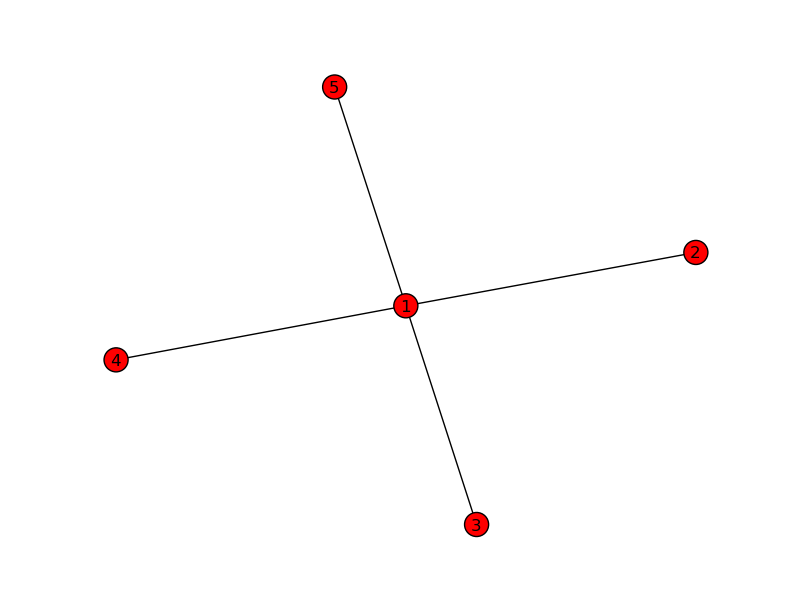
\includegraphics[width=0.5\textwidth]{degree_example}
\end{figure}

Closeness Centrality:
	Ability to move information from one side of the network to another (i.e., gossip) is an important step towards establishing a shared perception of the world—whether it has to do with someone’s choice of outfits at a party or the formation of a political movement. 

Thus, distance to others (or the inverse of it, closeness) can define a person’s role in 
the network. This principle is at the root of the closeness centrality metric—the next 
centrality concept we will explore. 
The calculation of closeness centrality is computationally expensive: 
1. Compute the shortest path between every pair of nodes using Dijkstra’s algorithm, 
and store these distances in a table. 
2. For every node: 
	a. Compute average distance to all other nodes 
	b. Divide by maximum distance 
	c. Closeness = 1 divided by average distance 

Betweenness centrality: It is based on the assumption that an individual may gain power 
if he presides over a communication bottleneck. In terms of computer network it could be thought of as the node, that if removed would result in two disjoint network.

The way we measure betweenness is as follows; this algorithm is fairly time-consuming 
for large networks: 
\begin{itemize}

\item Compute the shortest paths between every pair of nodes using Dijkstra's 
Algorithm. 
\item For every node I in the network: 
	 Count the number of shortest paths that I is on 
\item Normalize the numbers to bring your results to the 0-1 range. 
\end{itemize}


\begin{figure}[h]
\caption{Betweenness Centrality of 1 and 2 is higher that 5,6,3 and 4 since more no of shortest path pass through 1 and 2.}
\centering
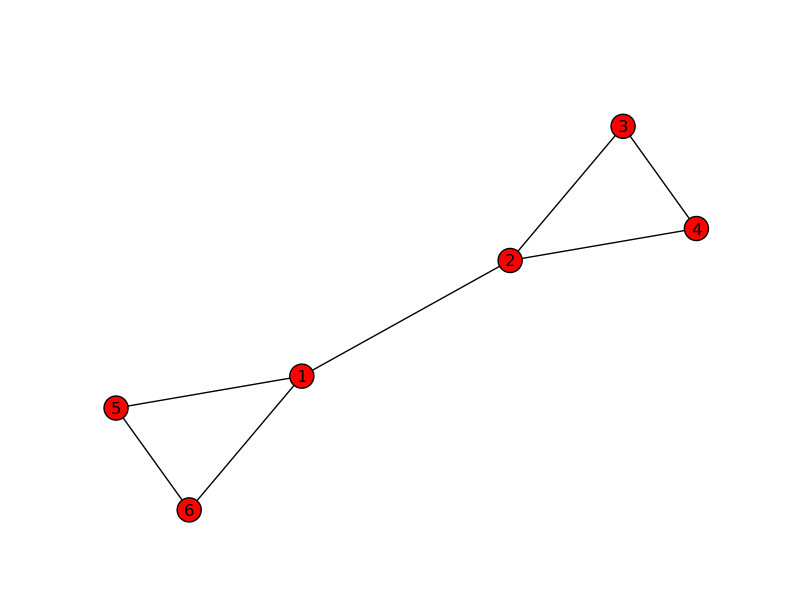
\includegraphics[width=0.5\textwidth]{betweeness_example}
\end{figure}

Simplified PageRank algorithm 

PageRank: is scaled between 0 and 1 and represents the likelihood that a person following links (i.e., traversing the network, “surfing” the web, etc) will arrive at a particular page or encounter a particular person. A 0.5 probability is commonly interpreted as a “50\% chance” of an event. Hence, a PageRank of 0.5 means there is a 50\% chance that a person clicking on a random link will be directed to the document with the 0.5 PageRank. 

\begin{figure}[h]
\caption{All the Nodes are assigned equal probability}
\centering
\includegraphics[width=0.5\textwidth]{pr1}
\end{figure}

Components and Subgraphs 
\begin{itemize}

\item subgraph is a subset of the nodes of a network, and all of the edges linking these nodes. Any group of nodes can form a subgraph—and further down we will describe several interesting ways to use this. 

\item Component subgraphs (or simply components) are portions of the network that are disconnected from each other. Before the meeting of Romeo and Juliet, the two families were quite separate (save for the conflict ties), and thus could be treated as components. 

\end{itemize}

\begin{figure}[h]
\caption{Facebook Network having 3 component}
\centering
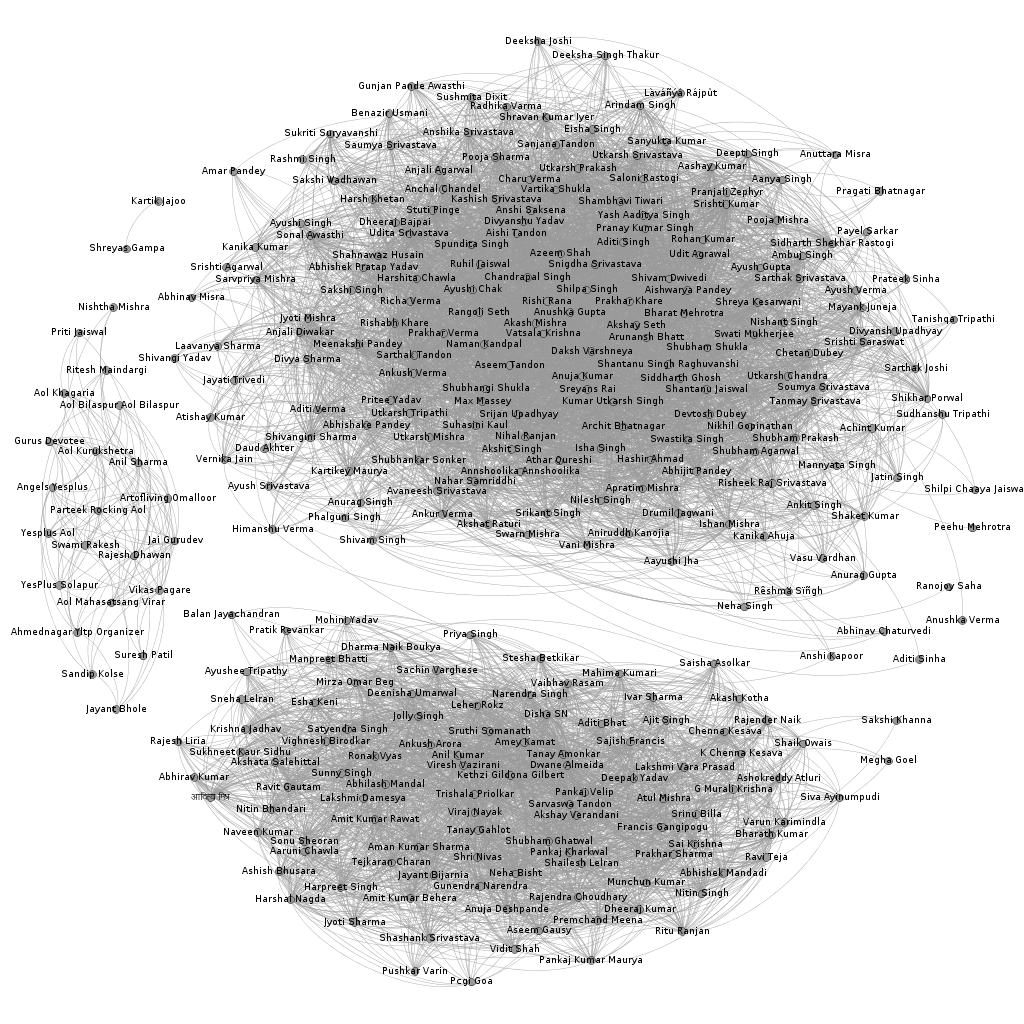
\includegraphics[width=0.5\textwidth]{component}
\end{figure}

Subgraphs—Ego Networks:Ego networks are sub-networks that are centered on a certain node. On Facebook and 
LinkedIn, these are simply described as “your network”—but you can only access your 
own ego networks, and can’t do a broader survey. Having a larger dataset allows us to 
survey and compare ego networks of various people. 


\begin{figure}[h]
\caption{Ego Graph of node “1” of radius 1}
\centering
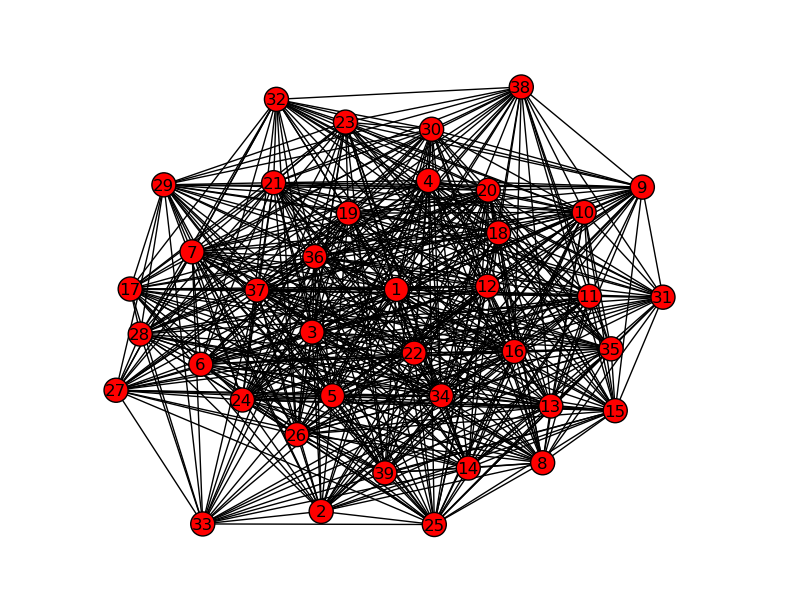
\includegraphics[width=0.5\textwidth]{ego_graph}
\end{figure}

Cliques:While we might have an intuitive understanding of a clique in a social network as a cohesive group of people that are tightly connected to each other (and not tightly connected to people outside the group), in the field of SNA there is a formal mathematical definition that is quite a bit more rigorous. A clique is defined as a maximal complete subgraph of a given graph—i.e., a group of people where everybody is connected directly to everyone else. The word “maximal” means that no other nodes can be added to the clique without making it less connected. Essentially, a clique consists of several overlapping closed triads, and inherits many of the culture-generating, and amplification properties of closed triads 
Multi Mode Network:Much of network data currently available comes in a 2-mode (or bimodal, or bipartite) 
format—that is, there are two different types of nodes, and links determine relation- 
ships between one set of nodes and the other. 
In the the graph given below “students” are connected to “college”,which is a of different type.
Such network are known as multi mode network since they contain two different type of entity connected together.

\begin{figure}[h]
\caption{Multimode network of people connected to NIT, Goa in my Facebook network.}
\centering
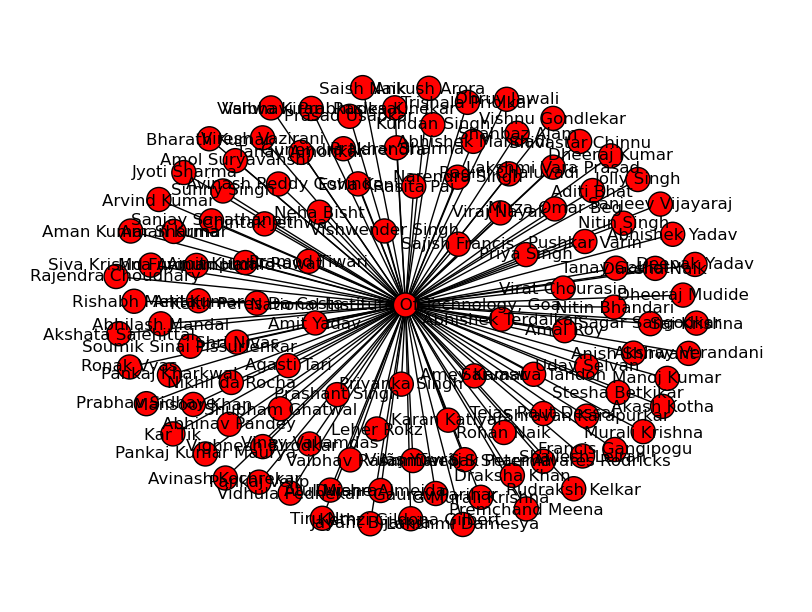
\includegraphics[width=0.5\textwidth]{multimode_nitg}
\end{figure}

How are tools mentioned above used in Targeted Advertisement:
Graph api is used to extract data from facebook about friends general information. Using this information a knowledge graph connecting interest subject with people is created. Then People who are interested in topic are identified using the multi mode graph so constructed using simple edge connection identification. Then interest subject is removed so that the graph comprises entirely of people.  Then sub component of the graphs are identified. Among these sub component people who are most influential are identified using centrality measure like degree, closeness , betweenness, page rank and HITS. 

\section{Real time information in disaster situation}

Quick Availability of information in disaster struck situation can speed up disaster rescue effort. Time after the disaster is the most critical time since majority of life can be saved. Therefore the strategy employed is very essential. Information about Survivor Position, Volunteer Position, Operational Clinics,  fuel station and road etc is very valuable in such scenario. 

I have designed a simulation of the request sent to a server after disaster scenario. Consider a disaster situation, survivor can give his/her real time position information to server. These request would look like this:

\begin{itemize}
\item SURVIVOR me1 (386 169) 
\item SURVIVOR me2 (163 128) 
\item SURVIVOR me3 (158 48) 
\item SURVIVOR me4 (158 90) 
\item SURVIVOR me5 (84 309) 
\item SURVIVOR me6 (260 17) 
\item SURVIVOR me7 (387 393) 
\item SURVIVOR me8 (319 332) 
\end{itemize}


In my simulation i have used python language for scripting and mongodb for database. For graphical simulation  Tkinter library is used. 


In this simulation humans are represented by class Person. Survivor are represented as Survivor class which inherits properties of a person. Volunteer also inherits from Person. Person has two attribute “Name” and “Location”. Location is stored as a “Point” object and “Name” is a string.
The disaster struck area is abstracted as Cartesian field. In Field the survivor pops up with probability “ppop”. Volunteer pops with a probability one tenth of ppop. This makes the game interesting since the resources are constraint, therefore strategy of moving Volunteer must be optimal.

At each time step the field is updated and new survivor is added. These changes are made to database. Position of volunteer and presence of survivor is also tested to maintain consistency between database and program objects. Volunteer are redrawn at each time step to account for change in their position. Survivor are deleted based on the changes made to database and volunteer position.

Player uses another script to make changes to Volunteer position depending upon the amount of data available to him. There are two modes of game-play:
\begin{itemize}
\item
 No information about survivor position is available to player.
\item
Survivor position can be queried according to certain function.
\end{itemize}
This play simulates the actual work done by Palantir Organization after Sandy Hurricane in NewYork, USA. Analytical tools were developed at runtime to suit the need. Network was established to connect volunteer with survivor.

PALANTIR’S SOLUTION:Palantir sent several engineers to camp out at Team Rubicon’s command center in the Rockaways. There, they partnered with team leaders to develop an application that enabled volunteers to enter requests for assistance into Palantir Gotham through web-enabled mobile devices. Within days, 
volunteers on the ground were using iPads and smart phones to file requests for water, medical supplies, and home repairs in Palantir Gotham, where they were aggregated and analyzed as part of Team Rubicon’s broader operation. Volunteers also used the mobile devices to capture photos of 
flooded spaces, damaged buildings, and blocked roads, which were entered into Palantir Gotham as media objects and used to inform response planning. 
Analysts at Team Rubicon’s command center used Palantir Gotham to maintain situational awareness across all response activities. Coordinators tracked volunteer progress and dispatched additional support as needed. Analysts at Team Rubicon’s command center also used Palantir to connect to data sources provided by other organizations, including information on fuel availability, power grids, and available medical clinics. Volunteers on the ground accessed this information using Palantir and relayed the information to affected individuals. Using Palantir Gotham’s Map application, dispatchers could see where volunteers were located in relation to damaged houses

\section{Freakonomics}
Knowing what to measure and how to measure it helps in uncovering the hidden side of everything. Conventional wisdom is not always right.This means that decision based on our institution(which are formed by conventional wisdom) can get us into trouble. This is where data comes in. Through out the book Freakonomics Hypothesis is tested against data. This has helped in validating some hypothesis while scraping others.

	Economics at its core is study of incentives. Incentives are powerful bullet that can change situations. Consider the case of day care center in Haifa, Israel where bunch of economist conducted a study on incentives. Workers at center had to wait for parents who came late. In order to curb this they kept a fee of 3. Result? More no of parents started coming late!.
	This is where decision on conventional wisdom can back fire. Lets see why Decision on conventional wisdom was wrong, and how it could have been avoided. Incentives are classified into three categories:
\begin{itemize}
\item Moral:The reason why parents avoided coming late was of moral incentives
\item Economic:Heavy tax on liquor is an Economic incentive.
\item Social: Prostitute hide their profession of Social incentives
\end{itemize}

No of parents that came late increased because new fine gave economic incentive and reduced  moral incentive.
Study of Freakonomics takes non intuitive questions like:
\begin{itemize}
\item Why should suicide bomber buy life insurance
\item Is altruism real?
\item Is Global Warming over hyped?
\item Whats common between school teacher and sumo wrestler?
\item Why are expert so often wrong?
\item How much parent matter in success of child?
\item Why do Drug Dealer Live with their mom?
\end{itemize}

All of the above will yield wrong answer if one uses his intuitions to answer them. These question require data against which hypothesis can be tested. 

Since Steven D.Levitt(Author of Freakonomics) is an American Author, all his study were based in US. But the essence of the book was universal ie:

“Conventional Wisdom is most often wrong!”
“People respond to incentive”
“Things can have distant and subtle cause”

Freakonomics study has huge implication in policy formulation by government. Consider the case of Food Security bill that was passed recently, though it has noble intention, its not economically sound. Major problem in Food distribution system still remain unaddressed. If policy implication aren't tested and launched through out the country, it would create corruption and further aggravate the problem. Such kind of policy can have unintended consequences.

\section{Conclusion}

\section{Reference}


\end{document}

